%iffalse
\let\negmedspace\undefined
\let\negthickspace\undefined
\documentclass[journal,12pt,onecolumn]{IEEEtran}
\usepackage{pgfplots}
\usepackage{cite}
\usepackage{amsmath,amssymb,amsfonts,amsthm}
\usepackage{algorithmic}
\usepackage{graphicx}
\usepackage{textcomp}
\usepackage{xcolor}
\usepackage{txfonts}
\usepackage{listings}
\usepackage{enumitem}
\usepackage{mathtools}
\usepackage{gensymb}
\usepackage{comment}
\usepackage[breaklinks=true]{hyperref}
\usepackage{tkz-euclide} 
\usepackage{listings}
\usepackage{gvv}                                        
%\def\inputGnumericTable{}                                 
\usepackage[latin1]{inputenc}                                
\usepackage{color}                                            
\usepackage{array}                                            
\usepackage{longtable}                                       
\usepackage{calc}                                             
\usepackage{multirow}                                         
\usepackage{hhline}                                           
\usepackage{ifthen}                                           
\usepackage{lscape}
\usepackage{tabularx}
\usepackage{array}
\usepackage{float}
\usepackage{circuitikz}
\newtheorem{theorem}{Theorem}[section]
\newtheorem{problem}{Problem}
\newtheorem{proposition}{Proposition}[section]
\newtheorem{lemma}{Lemma}[section]
\newtheorem{corollary}[theorem]{Corollary}
\newtheorem{example}{Example}[section]
\newtheorem{definition}[problem]{Definition}
\newcommand{\BEQA}{\begin{eqnarray}}
\newcommand{\EEQA}{\end{eqnarray}}
\newcommand{\define}{\stackrel{\triangle}{=}}
\theoremstyle{remark}
\newtheorem{rem}{Remark}

% Marks the beginning of the document
\begin{document}
\bibliographystyle{IEEEtran}
\vspace{3cm}

\title{2017-ME-'53-65'}
\author{AI24BTECH11013-Geetha charani}
\maketitle
\bigskip

\renewcommand{\thefigure}{\theenumi}
\renewcommand{\thetable}{\theenumi}
\begin{enumerate}
\item A block of length 200 mm is machined by a slab milling cutter 34 mm in diameter. The depth of cut and table feed are set at 2 mm and 18 mm/minute, repectively. Considering the approach and the over travel of the cutter to be same, the minimum estimated machining time per pass is $\underline{\hspace{2cm}}$ minutes.
\item A sprue in a sand mould has a top diameter of 20 mm and height of 200 mm. The velocity of the molten metal at the entry of the sprue is 0.5m/s. Assume acceleration due to gravity as $9.8 m/{s}^2$ and neglect all looses. If the mould is well ventilated, the velocity $\brak{upto 3 decimal points accuracy}$ of the molten metal at the bottom of the sprue is $\underline{\hspace{2 cm}}$ m/s.
\item Two cutting tools with tool life equations given below are being compared:\\
Tool 1: $VT^{0.1} = 150$\\
Tool 2:$VT^{0.3} 300$\\
where V is cutting spped in m/minute and T is tool life in minutes. The breakeven cutting speed beyond which Tool 2 will have a higher tool life is $\underline{\hspace{2 cm}}$ m/minute.
\item He was one of my best $\underline{\hspace{2 cm}}$ and I felt his loss $\underline{\hspace{2 cm}}$.
\begin{enumerate}
    \item friend, keenly
    \item friends, keen 
    \item friend, keener 
    \item friends, keenly
\end{enumerate}
\item As the two speakers became increasingly agitated, the debate becomes $\underline{\hspace{2 cm}}$.
\begin{enumerate}
    \item lukewarm
    \item poetic 
    \item forgiving
    \item heated
\end{enumerate}
\item A right-angled cone \brak{with base radius 5 cm and height 12 cm}, as shown in the figure below, is rolled on the ground keeping the point P fixed until the point Q \brak{at the base of the cone, as shown} touches the ground again
\begin{figure}[!ht]
\centering
\resizebox{0.3\textwidth}{!}{%
\begin{circuitikz}
\tikzstyle{every node}=[font=\small]
\draw [short] (7.25,9.25) -- (18,9.25);
\draw [short] (9,12.75) -- (13.5,9.25);
\draw [ rotate around={-31:(8,11)}] (8,11) ellipse (1cm and 2cm);
\draw [dashed] (13.5,9.25) -- (8,11);
\draw [dashed] (8,11) -- (9,12.75);
\draw (13.25,14.25) to[short] (13.25,9.75);
\draw [->, >=Stealth] (12.25,13.75) .. controls (13,13) and (13.5,13) .. (14.25,13.25) ;
\draw [->, >=Stealth] (6.5,12.5) .. controls (7.5,14) and (8.5,14) .. (10,13.25) ;
\node [font=\small, rotate around={31:(0,0)}] at (7.5,14) {360 deg.};
\node [font=\small] at (14,12.75) {?};
\node [font=\small, rotate around={63:(0,0)}] at (8.25,11.75) {r=5cm};
\node [font=\small, rotate around={-19:(0,0)}] at (10.5,10.5) {h=12cm};
\node at (7.25,9.25) [circ] {};
\node [font=\small] at (7.25,9.5) {O};
\node [font=\small] at (13.5,9) {P};
\end{circuitikz}
}%

\label{fig:my_label}
\end{figure}
By what angle $\brak{in radius}$ about P does the cone travel?
\begin{enumerate}
    \item $\frac{5\pi}{12}$
    \item $\frac{5\pi}{24}$
    \item $\frac{24\pi}{5}$
    \item $\frac{10\pi}{13}$
\end{enumerate}
\item In a company with 100 employees, 45 earn Rs.20,000 per month, 25 earn R. 30,000, 20 earn Rs. 40,000, 8 earn Rs. 60,000, and 2 earn Rs. 150,000. The median of the salaries is 
\begin{enumerate}
    \item Rs. 20,000
    \item Rs. 30,000
    \item Rs. 32,300
    \item Rs. 40,000
\end{enumerate}
\item P, Q, and R talk about S's car collection. P states that S has at least 3 cars. Q believes that S has less than 3 cars. R indicates that to his knowledge, S has at least one car. Only one of P, Q and R is 
\begin{enumerate}
    \item 0
    \item 1
    \item 3
    \item Cannot be determined
\end{enumerate}
\item "Here, throughout the early 1820s, Stuart continued to fight his losing battle to allow his sepoys to wear their caste-marks and their own choice of facial hair on parade, being again reprimanded by the commander-in-chief. His retort that 'A stronger instance than this of European prejudice with relation to this country has never come under my observations' had no effect on his superiors."

According to this paragraph, which of the statements below is most accurate?
\begin{enumerate}
    \item Stuart's commander-in-chief was moved by this demonstration of his prejudice.
    \item The Europeans were accommodating of the sepoys' desire to wear their caste-marks. 
    \item Stuart's 'losing battle refers to his inability to succeed in enabling sepoys to wear caste-marks.
    \item The commander-in-chief was exempt from the European prejudice that dictated how the sepoys were to dress.
\end{enumerate}
\item What is the sum of the missing digits in the subtraction problem below?\\
\begin{figure}[!ht]
\centering
\resizebox{0.3\textwidth}{!}{%
\begin{circuitikz}
\tikzstyle{every node}=[font=\large]
\node [font=\large] at (8.25,12.25) {5};
\draw (8.75,12) to[short] (9.25,12);
\draw (9.5,12) to[short] (10,12);
\draw (10.25,12) to[short] (10.75,12);
\draw (11,12) to[short] (11.5,12);
\draw (7.25,11.25) to[short] (7.75,11.25);
\draw (9.5,11) to[short] (10,11);
\node [font=\large] at (8.25,11.25) {4};
\node [font=\large] at (9,11.25) {8};
\node [font=\large] at (10.5,11.25) {8};
\node [font=\large] at (11.25,11.25) {9};
\draw (7,10.5) to[short] (13,10.5);
\node [font=\large] at (9,9.75) {1};
\node [font=\large] at (10,9.75) {1};
\node [font=\large] at (10.75,9.75) {1};
\node [font=\large] at (11.5,9.75) {1};
\end{circuitikz}
}%

\label{fig:my_label}
\end{figure}
\begin{enumerate}
    \item 8
    \item 10
    \item 11
    \item Cannot be determined
\end{enumerate}
\item Let $S_1$ be the plane figure consisting of the points $\brak{x, y}$ given by the inequalities $|x-1| \leq 2$ and $|y+2|\leq 3$. Let $S_2$ be the plane figure by the inequalities $x-y \geq -2, y \geq 1$, and $x \leq 3$. Let S be the union of $S_1$ and $S_2$. The area of S is
\begin{enumerate}
    \item 26
    \item 28
    \item 32
    \item 34
\end{enumerate}
\item Two very famous sportsmen Mark and Steve happened to be brothers, and played for country K. Mark teased James, an opponent from country E. "There is no way you are good enough to play for your country." James replied, "Maybe not, but at least I am the best player in my own family."

Which one of the following can be inferred from this conversation?
\begin{enumerate}
    \item Mark was known to play better than James
    \item Steve was known to play better than Mark 
    \item James and Steve were good friends
    \item James played better than Steve
\end{enumerate}
\item The growth of bacteria (lactobacillus) in milk leads to curd formation. A minimum bacterial population density of 0.8 (in suitable units) is needed to form curd. In the graph below, the population density of lactobacillus in 1 liter of milk is plotted as a function of time, at two different temperatures, 25 $^{0}C$ and 37 $^{0}C$\\

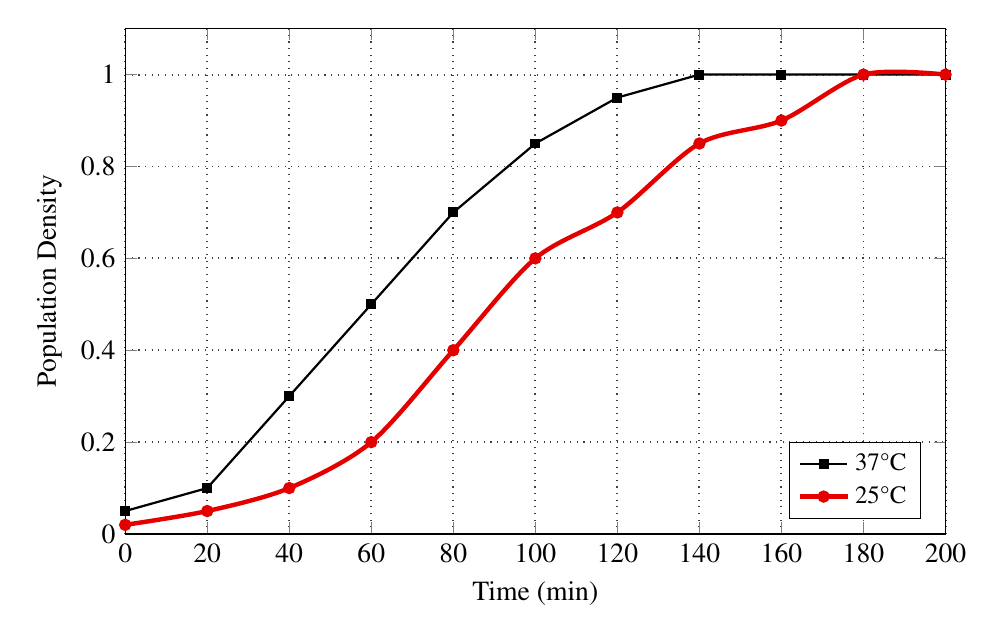
\begin{tikzpicture}
    \begin{axis}[
        width=12cm,
        height=8cm,
        xlabel={Time (min)},
        ylabel={Population Density},
        xmin=0, xmax=200,
        ymin=0, ymax=1.1,
        xtick={0, 20, 40, 60, 80, 100, 120, 140, 160, 180, 200},
        ytick={0, 0.2, 0.4, 0.6, 0.8, 1.0},
        legend pos=south east,
        grid=both,
        grid style={dotted, darkgray, line width=0.7pt}, % Darker dotted lines
        legend style={font=\small},
        legend cell align={left},
    ]

    % 37°C curve
    \addplot[
        color=black,
        mark=square*,
        mark options={scale=0.7, fill=black},
        thick
    ]
    coordinates {
        (0, 0.05) (20, 0.1) (40, 0.3) (60, 0.5) (80, 0.7) (100, 0.85) (120, 0.95) (140, 1.0) (160, 1.0) (180, 1.0) (200, 1.0)
    };
    \addlegendentry{37°C}

    % 25°C curve (smoothed and bolder red)
    \addplot[
        color=red!90!black, % Darker shade of red
        mark=*,
        mark options={scale=0.7, fill=red!90!black},
        ultra thick, % Thicker line for clarity
        smooth % Makes the line a smooth curve
    ]
    coordinates {
        (0, 0.02) (20, 0.05) (40, 0.1) (60, 0.2) (80, 0.4) (100, 0.6) (120, 0.7) (140, 0.85) (160, 0.9) (180, 1.0) (200, 1.0)
    };
    \addlegendentry{25°C}

    \end{axis}
\end{tikzpicture}

Consider the following statements based on the data shown above:

i. The growth in bacterial population stops earlier at 37 $^{0}$C as compared to 25 $^{0}$C.\\
ii. The time taken for curd formation at 25 $^{0}$C is twice time taken at 37 $^{0}$C
Which one of the following options is correct?
\begin{enumerate}
    \item Only i
    \item Only ii
    \item Both i and ii
    \item Neither i nor ii
\end{enumerate}
\end{enumerate}
\end{document}

